\newpage
\section{Appendix / supplemental material}


\subsection{Broader Impacts}\label{sec:broader_impacts}

The broader impacts of our novel multi-modal image generation model extend across various domains and societal aspects. Here, we provide a comprehensive reflection on the potential implications and ethical considerations associated with our advancements in conditional image generation.

\textbf{Impact on Creative Industries}: The ability to generate images from text and additional modalities can revolutionize various creative industries, from graphic design to film and gaming. While this may lead to concerns about job displacement, we anticipate that our model will primarily serve as a tool to augment the creative process, allowing professionals to achieve greater efficiency and explore new artistic frontiers.

\textbf{Accessibility and Empowerment}: By enabling the generation of high-fidelity images based on textual descriptions, our model can democratize the creation of visual content. This empowers individuals, including those without specialized artistic skills, to bring their ideas to life. We aim to make our technology accessible to a wide range of users, fostering creativity and innovation.

\textbf{Education and Research}: Our model can be a powerful educational tool, providing students and researchers with a means to visualize complex concepts and data. It can also facilitate scientific discovery by generating images that aid in the understanding of abstract or theoretical concepts, thereby enhancing learning and research outcomes.

\textbf{Ethical Use of Technology}: The potential for misuse of image generation technology, such as creating deepfakes or manipulating visual content for deceptive purposes, is a significant concern. We are dedicated to promoting the ethical use of our technology and are actively developing safeguards against such misuse. This includes:

\begin{itemize}
\item Watermarking and Traceability: Implementing features that allow the traceability of generated images, preventing unauthorized use and ensuring accountability.

\item Ethical Guidelines: Establishing clear guidelines for the ethical use of our model, emphasizing the importance of transparency and honesty in the generation and dissemination of images.

\item Collaboration with Stakeholders: Engaging with artists, content creators, and legal experts to develop a robust framework that protects intellectual property and ensures fair use.

\item Public Awareness: Educating the public about the capabilities and limitations of our technology, promoting responsible use and critical thinking regarding the authenticity of visual content.

\end{itemize}

\textbf{Environmental Considerations}: We are cognizant of the environmental impact associated with the computational requirements of AI models. Our approach to feature integration and the use of time embeddings aim to reduce the computational footprint, aligning with our commitment to sustainable AI development.

In conclusion, while our multi-modal image generation model presents exciting opportunities for innovation and creativity, it also comes with a set of ethical and societal responsibilities. We are dedicated to addressing these challenges proactively, ensuring that our technology is developed and used in a manner that is beneficial, responsible, and respectful of diverse societal values.

\subsection{Safeguards}\label{sec:safeguards}
\begin{enumerate}
    \item During training, our model utilized Stable Diffusion 1.5 which is capable of detecting NFSW content. This could prevent our model from generating and learning NFSW images. 
    \item The source of our internal dataset could guarantee that there is not any NFSW content. 
\end{enumerate}

\subsection{License}\label{sec:license}
\begin{enumerate}
    \item Stable Diffusion 1.5:  The CreativeML OpenRAIL M license.
    \item LAION: MIT License.
    \item COYO: CC-BY-4.0 License. 
    \item ELLA: Apache-2.0 license.
\end{enumerate}

\subsection{More visualization}

More visualization using portrait condition is shown in Figure~\ref{fig:supplymentary}. We show portrait generation results for both males and females. They all share the same generation prompts as those in Figure~\ref{fig:teaser}.

The prompts are listed below:
\begin{enumerate}
    \item A person sits on a checked picnic blanket in the lush, green park, surrounded by blooming wildflowers and tall trees. She is enjoying her breakfast, which consists of a toasted bagel with cream cheese and a steaming cup of coffee while reading a newspaper held delicately in her hand. The sun peeks through the branches, casting dappled shadows across the scene.
    \item a person is deeply engrossed in her artistic endeavor within a serene park surrounded by blossoming wildflowers and towering trees. The painting, a vivid portrayal of the park's essence, captures the interplay of light and shadow as the sun's rays dance through the foliage above. The tranquil setting enhances her focus, as the natural beauty of the park becomes an integral part of her creation.
    \item In the heart of a sunlit park, a person is playing guitar. Around her, vibrant pink cherry blossoms bloom profusely from their branches, creating a canopy of soft, delicate petals overhead. The lush green grass below is sprinkled with a tapestry of multi-colored wildflowers swaying gently in the breeze. A few nearby benches invite passersby to pause and enjoy the harmonious blend of nature and music. 
\end{enumerate}

\begin{figure}[t]
    \centering
    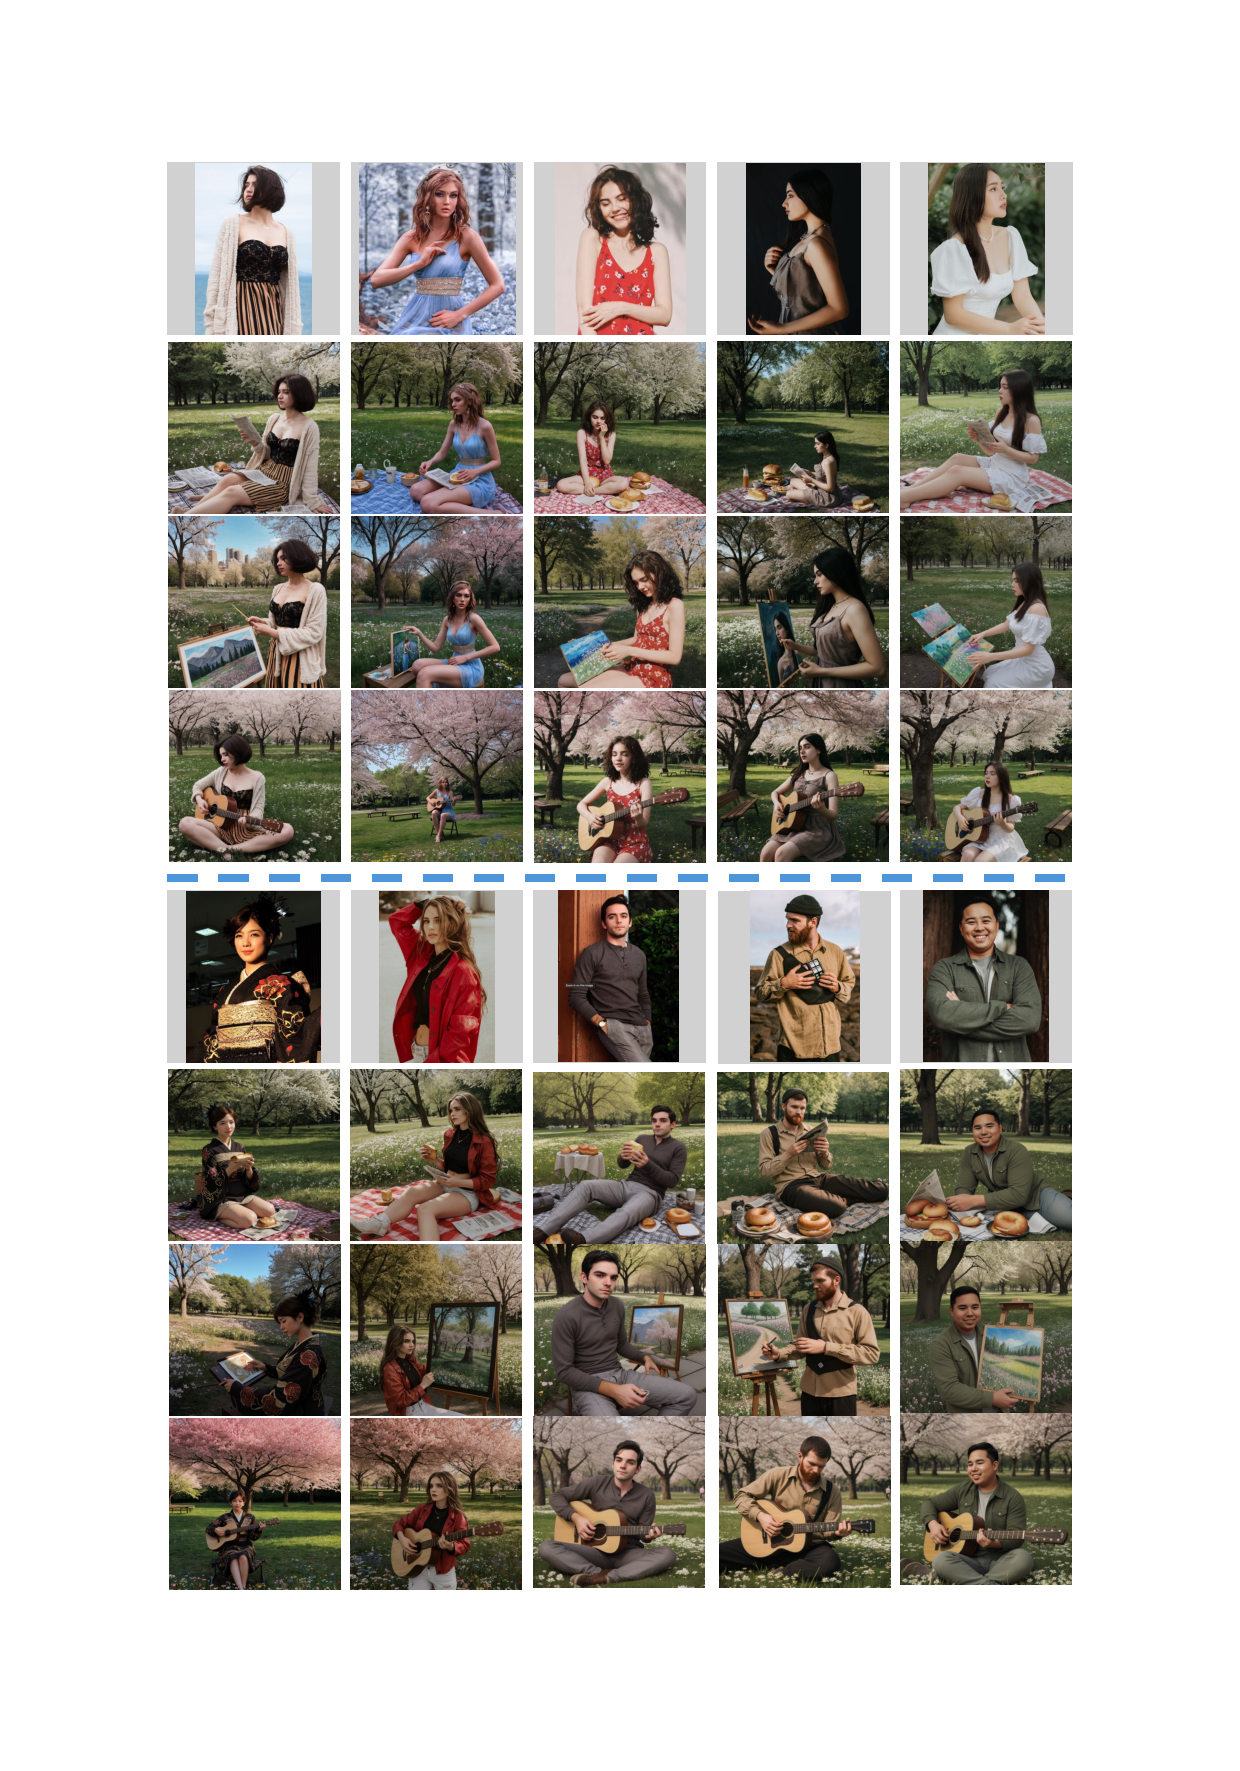
\includegraphics[width=0.95\textwidth]{images/supplymentary.pdf}
    \caption{Illustration of more portrait generation examples. The first row is the condition image, and the following rows show the results of EMMA. The prompts for those examples are listed in our Appendix.}
    \label{fig:supplymentary}
\end{figure}
\begin{figure}[t]
    \centering
    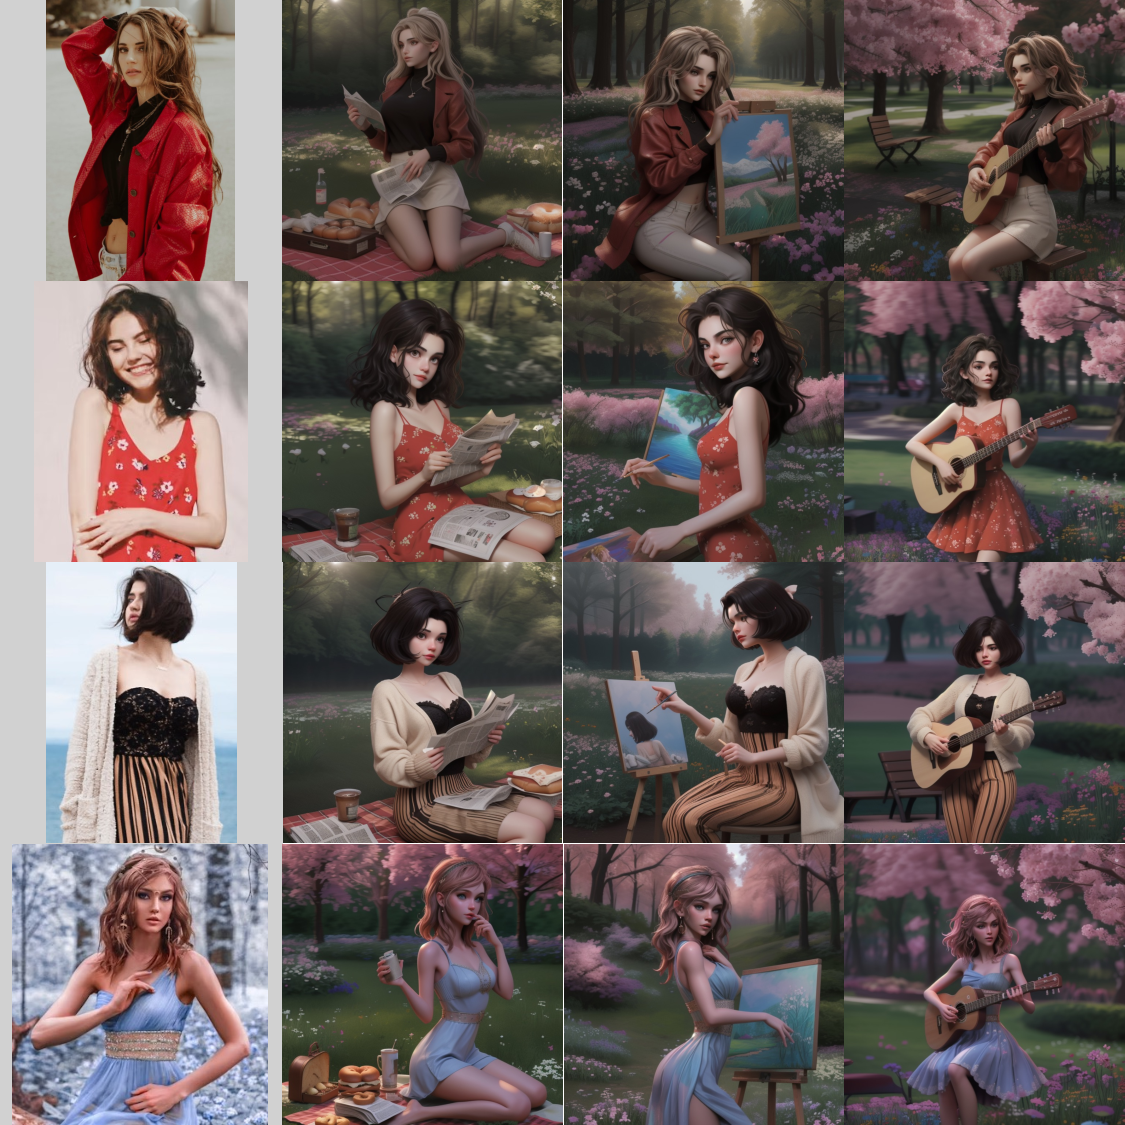
\includegraphics[width=0.9\textwidth]{images/supplymentary_toonyou.pdf}
    \caption{Generated results using EMMA and ToonYou's U-net. The first column is the condition image, and the following columns show the corresponding generated results. The prompts are also the same as Figure~\ref{fig:supplymentary}.}
    \label{fig:supplymentary_toonyou}
\end{figure}
\begin{figure}[t]
    \centering
    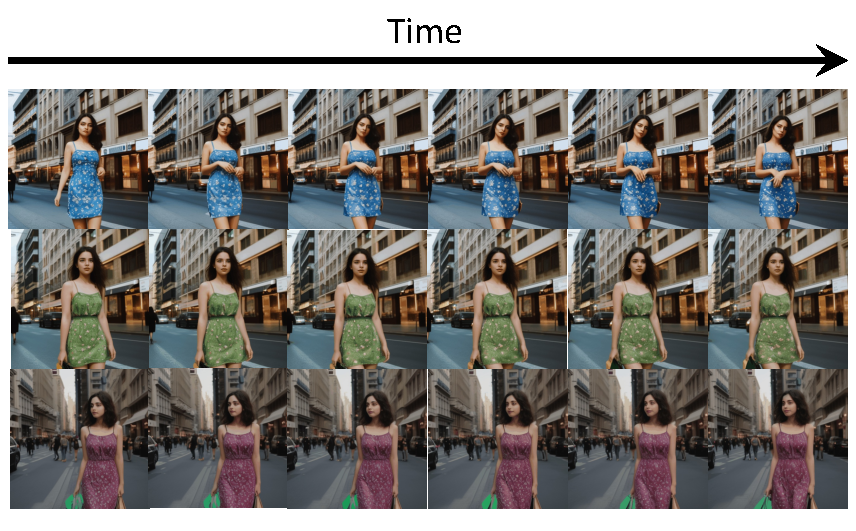
\includegraphics[width=0.9\textwidth]{images/supplymentary_video.pdf}
    \caption{Generated results using EMMA and AnimateDiff's U-net. The conditional image and prompts are shown in Figure~\ref{fig:teaser}. }
    \label{fig:supplymentary_video}
\end{figure}

\subsection{Adaptation to existing extensions in community.} 
Since our proposed EMMA does not require training the diffusion models, we can utilize commonly used community-based diffusion models trained on CLIP text features, such as the picXreal and ToonYou models, which are representative of portrait and anime styles, respectively. Furthermore, our model can even be transferred to results from models like animatediff, which are secondary developments based on diffusion models. The results on these open-source communities are illustrated in Figure~\ref{fig:supplymentary_toonyou} and Figure~\ref{fig:supplymentary_video}.

\subsection{More Training Details}

\subsubsection{Training Settings for Different Conditions}
\paragraph{Text features plus common object features.} We train the model on our collected common object dataset for 200K iterations. The image feature extractor is CLIP-H/14, and we send both the global features and local features as the key and value features for cross-attention. The weights of this model also work as the initialization for the models conditioned on text features plus portrait features. 

\paragraph{Text features plus style features.} The model is trained on the common object dataset. The image features are also collected by CLIP-H/14 but only use the global features. The image features are then projected to 4 tokens by an extra linear layer. All the data processing procedures follow the IP-Adapter \cite{ye2023ip}.

\paragraph{Text features plus face features.} The model is trained on our own collected facial dataset for 200K iterations. We first detect and use only the face area for feature processing. Then we use AdaFace~\cite{kim2022adaface} for feature extraction and use them as the key and value features.

\subsubsection{More Ablations}

\textbf{Freeze Perceiver Resamplers.} Freezing the Perceiver Resamplers is an essential method for constructing effective multi-modal guidance. During training, we freeze the parameters of Perceiver Resamplers to keep the text following ability. Not freezing these layers will make it impossible for the composite of different EMMA models.

\textbf{Different assemble methods.} 
Our EMMA architecture enables the fusion of models from different conditions to form new models. Since these models do not require training, how to merge them becomes a question worth designing and contemplating. In addition to the combination methods outlined in our paper, such as those in formulas 3 and 4, we have designed several groups of results. Experimental results demonstrate that our method can significantly better integrate model characteristics. The way we merge models is also significantly related to the distinct patterns in the distribution of gate values.

\textbf{Object-centric mask.} During training and inference, we add an object-centric mask to avoid the influence of background image information.



\clearpage

